\documentclass[12pt]{article}
\usepackage{lgrind}
\usepackage{fullpage}
\usepackage{graphicx}
\usepackage{xtab}

\author{Bo Shi}
\title{6.111 Lab 2 Report \\ Design and Implementation of Main/Side Street Traffic Light Controller}
\date{October 13, 2004}


\begin{document}

\begin{titlepage}
\pagestyle{empty}
\maketitle

\begin{abstract}
This report details the design and implementation of a relatively simple
traffic light controller.  The intersection for which this controller is being
designed also has a walk lamp and traffic sensor (along one street).  A traffic
light system is composed of a relatively simple finite state machine and more
complicated timing modules that provide the finite state machine with start and
end pulses and also must be able to be programmed by traffic authorities.  The
testing process for this lab highlights the strengths and weaknesses of
simulation and functional testing as debugging methodologies.  In particular,
simulation is a good tool for diagnosing problems but only functional testing
can reveal particularly small timing errors which may hugely impact the system.
\end{abstract}
\end{titlepage}


\pagestyle{plain}
\pagenumbering{roman}
\setcounter{page}{1}
\tableofcontents

\newpage
\listoffigures 
\listoftables 

\newpage
\pagenumbering{arabic}
\setcounter{page}{1}
\section{Design Overview}
	\subsection{Requirements}
	This documents details the design for a traffic light controller at the
	intersection of Main Street and Side Street.  Both street lights are
	capable of sending a red, yellow, and green signal.  A walk signal is also
	available for pedestrians.  When the walk signal is on, all vehicle is
	halted.  A sensor is installed on Side street to monitor traffic.  The
	timing for each set of light signals depends on two things --- the values
	programmed into the controller by user input, and traffic conditions on
	Side Street.  If Side street has heavy traffic, Main Street's green signal
	length is shortened.  Conversely, Side street's green signal is lengthened
	under heavy traffic conditions.

	\subsection{Top Level Design}

	\begin{figure}[ht]
	\centering
	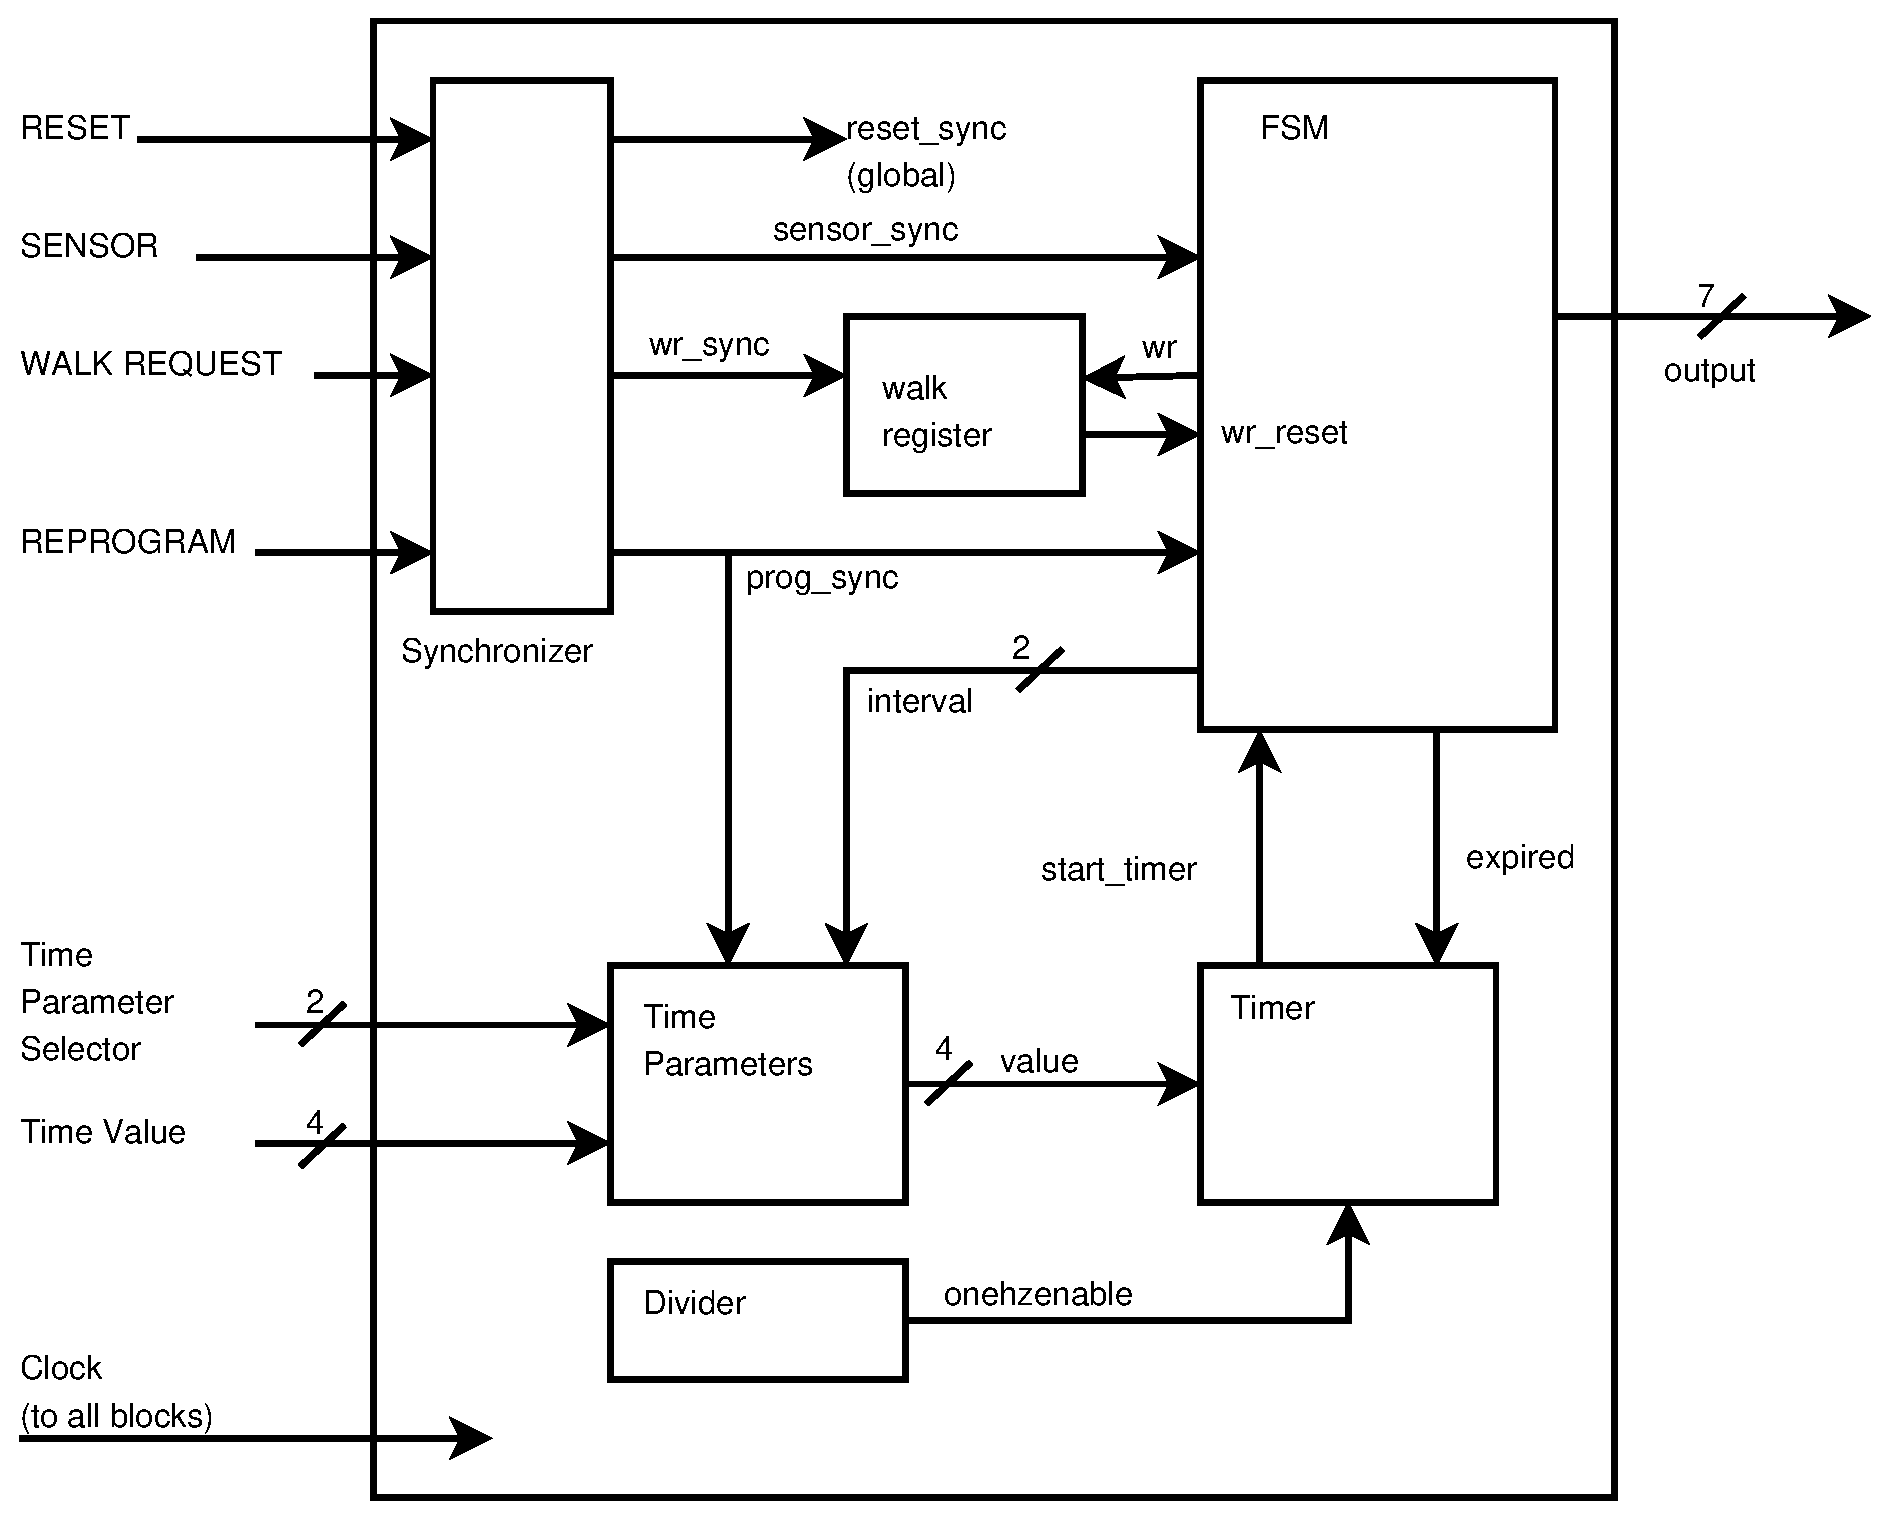
\includegraphics[scale=0.4]{block.ps}
	\caption{Block diagram of the modules inside the traffic light controller.}
	\label{fig:block}
	\end{figure}

	\begin{table}[ht]
	\caption[Output Setup]{Output setup:  the output pins are all connected to
	LED's}
	\centering
		\begin{tabular}{|c|c|c|c|c|c|c|}
		\hline
		Bit 6 & Bit 5 & Bit 4 & Bit 3 & Bit 2 & Bit 1 & Bit 0 \\ \hline
		Main Red & Main Yellow & Main Green & Side Red & Side Yellow & Side Green & Walk \\ \hline
		\end{tabular}
	\label{tbl:output}
	\end{table}


	The Finite State machine (FSM) handles all the control signals.  Each state in
	the FSM has an associated output controlling the traffic lights (i.e. when
	the Main street light is green or yellow, then the Side street light is red).
	The timer notifies the FSM when the time is appropriate to change states.
	The timer module receives data from the time parameter module.  The time
	parameter module stores the appropriate time intervals for a given state.


	The FPGA used is an Altera Flex 10K10
	clocked with a 1.8432--Mhz crystal oscillator.
	In addition to the clock input, the traffic light controller accepts four
	asynchronous inputs and two 2-bit and 4-bit synchronized inputs and has a
	seven-bit output controlling the switching of the traffic lights and the
	walk signal.  Figure ~\ref{fig:block} shows the input signals.  The four
	asynchronous inputs are tied to four push buttons which, upon being
	pressed,
	\begin{itemize}
		\item reset the traffic light controller (\texttt{RESET}),
		\item simulates traffic sensor input (\texttt{SENSOR}),
		\item notifies the FSM of a walk request (\texttt{WALK REQUEST}),
		\item reprograms the time intervals for a given signal (\texttt{REPROGRAM}).
	\end{itemize}

	The two synchronized inputs allow control over the duration that
	various states last (for example, one may change the duration of
	yellow-light intervals).  The input \texttt{TIME PARAMETER SELECTOR}
	selects the time interval to program and \texttt{TIME VALUE} sets
	the time value.  The output is a 7-bit value ordered as
	Table~\ref{tbl:output} shows.
	

\section{Module Implementation}
	\subsection{Walk Register}
	The specifications state that a walk signal can only occur after the
	Main street yellow light has expired.  As a consequence, when a walk
	light is requested, it is necessary to remember that such a request
	was made so that when the time is appropriate, the FSM will transition
	to the appropriate state that gives a walk signal.
	The walk register module has an internal bit that is set to high when a
	walk signal, \texttt{wr\_sync}, has been requested.  The \texttt{wr}
	output of the walk register module is held high until this request is
	honored.  When the FSM exits the \texttt{S\_walk} state, a
	\texttt{wr\_reset} pulse is sent by the FSM and the register is set to
	a value of zero.

	\subsection{Timer}
	Because there are different time intervals which are much longer than
	the time interval for a system clock cycle, this module is required to
	keep track of passing time and to signal the FSM when it should transition
	to a new state.
	The timer keeps an internal 4-bit counter.  The timer module is notified
	whenever 1 second elapses by a \texttt{onehzenable} pulse from the Divider
	module.  When it receives a \texttt{onehzenable} pulse from the divider
	module, the counter decrements.  When the counter's value is one, it sends
	out an {\texttt{expired}} pulse to the FSM.  Upon reception of a
	\texttt{start\_timer}
	pulse, the Timer will load a new counter value (the \texttt{value}
	signal) from the Time Parameter module and begin counting down.

	\subsection{Time Parameters}
	The duration of traffic light signals differs depending on the situation.
	Yellow lights are a warning, hence their duration is much shorter than
	other signals.
	This module maintains a table of integer values which represent
	the correct duration of a given state.  The data that this module
	provides is used by the timer module to count the duration of the FSM's
	current state so that it can notify the FSM to change state.  The timer
	module provides timing data according to the state of the FSM (through
	the 2-bit \texttt{interval} signal).  The default timing values are
	given in Table~\ref{tbl:timeparam}.

	The specification also states that the time parameters should be
	programmable.  On the \texttt{prog\_sync} pulse, the module will read
	the 4--bit time value (the input ``Time Value'' in
	Figure~\ref{fig:block} and program the interval selected by the 2--bit
	select signal.  It is assumed that these signals are in steady
	state when the reprogram button is pushed so that a synchronizer is not
	necessary. (the input ``Time Parameter Selector'').  It is possible
	that an error might cause a value of zero might be programmed as one of
	the time parameters.  Because the \texttt{expired} signal is only sent
	when the timer counter has value 1, a programmed value of zero will
	simply cause the time parameter to become 16 seconds long because the
	value in the register will wrap around to 0xF when 1 is
	subtracted from 0.

	\subsection{Divider}
	The time durations for each FSM state are measured and programmed in
	seconds.  A clock cycle for the system is significantly shorter than that.
	The divider sends a 1 hz pulse to other modules to keep track of time on a
	scale meaningful to humans.  The module keeps an internal counter 21-bits
	wide that increments each rising edge of the clock.  The clock used for the
	traffic light controller is a 1.8432 Mhz crystal oscillator so 1,843,200
	clock cycles is lasts approximately one second.  When the counter reaches
	the specified value of 1,843,200, the \texttt{onehzenable} pulse is sent.

	\begin{figure}
	\centering
	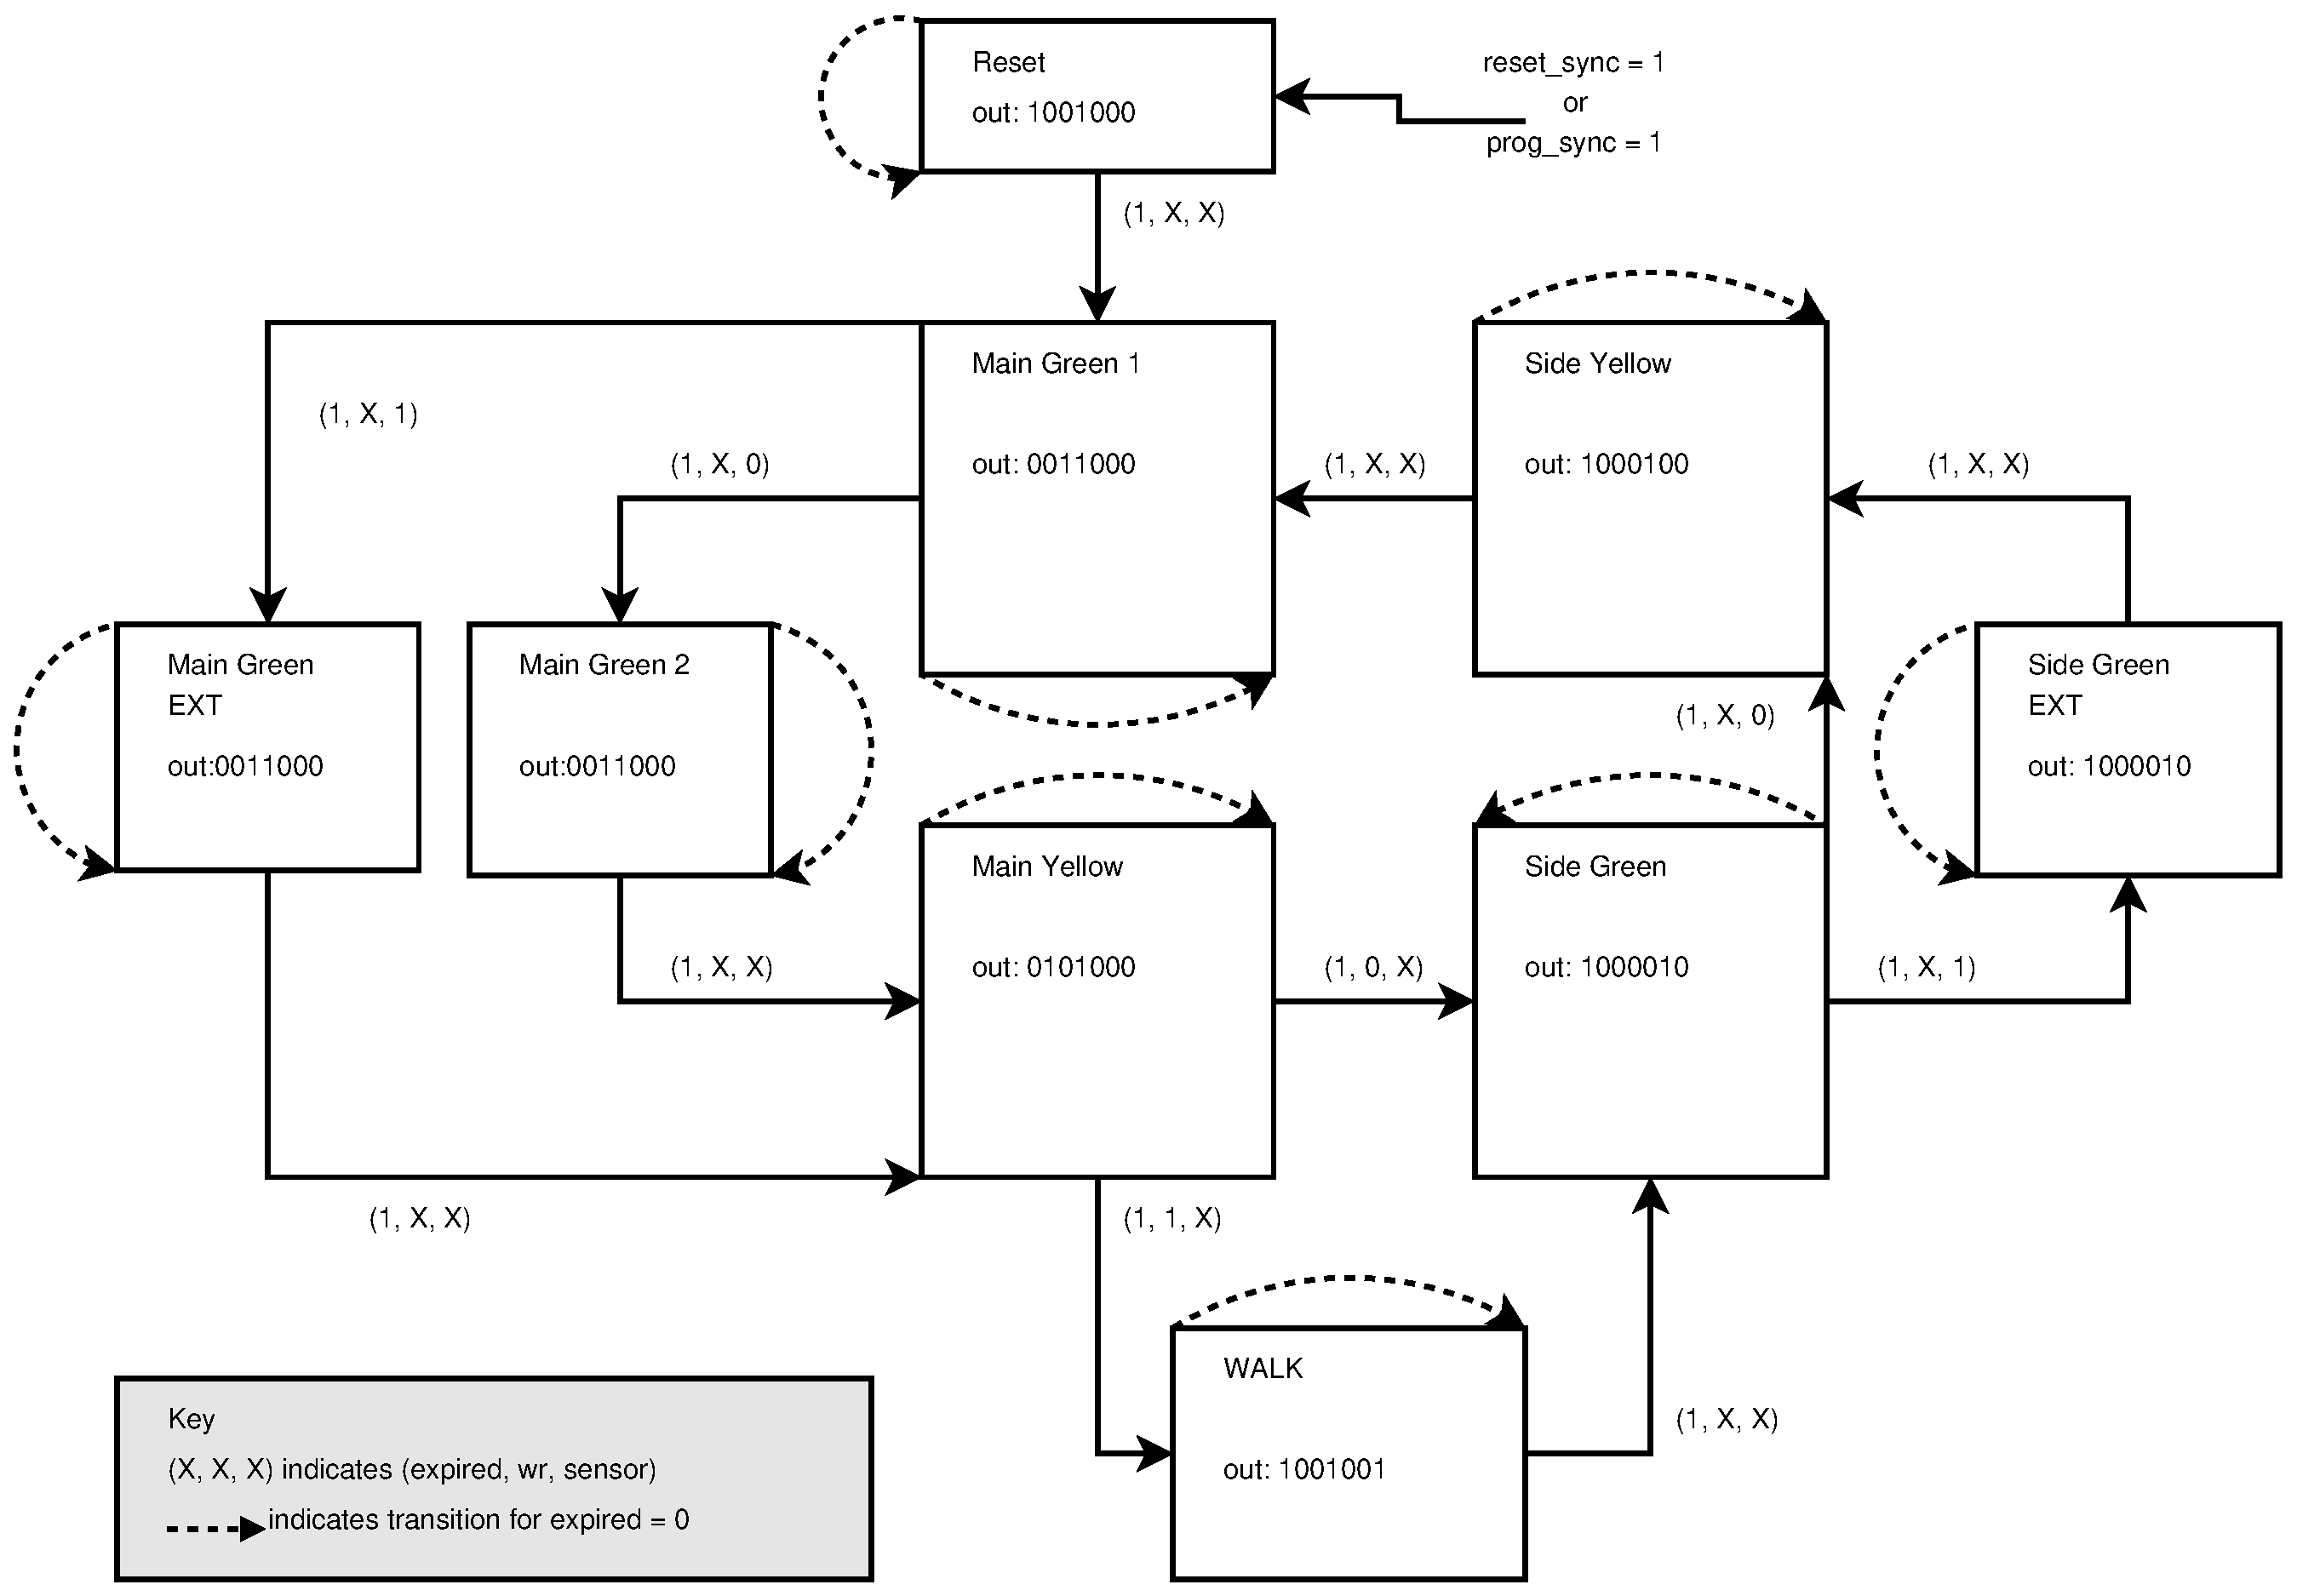
\includegraphics[scale=0.33]{fsm.ps}
	\caption[Finite State Machine for the Traffic Light Controller]
	{The original design used \texttt{S\_main\_green} as both
	the initial state and the reset state.  This was changed because the
	behavior of the design is not particularly safe.  If the reset were to
	be asserted during actual operation, it would be best to have a period
	of all red lights so that actual traffic does not get adversely
	confused.}
	\label{fig:fsm}
	\end{figure}

	\subsection{Finite State Machine}
	When RESET is asserted, the FSM enters the \texttt{S\_RESET}
	state.
	The \texttt{S\_RESET} state lasts for 3 seconds and then
	the controller starts normal operation.  As indicated by the state
	transition diagram (Figure~\ref{fig:fsm}), the default duration of Main Street's
	green light is $2 \cdot t_{base}$.  For Side Street, green signals will
	only last $t_{base}$ seconds. The default duration of any Yellow signal
	is $t_{ext}$.  The controller will behave normally unless the sensor
	detects traffic or a walk signal has been requested (\texttt{sensor} or
	\texttt{wr} signal is high).  In these cases, the new states will go
	according to what the state transition diagram shows;  a walk interval
	will occur \emph{only} after a Main Street yellow signal and the green signal
	will lengthen for Side Street or shorten for Main Street if the sensor
	detects traffic on Side Street.

	The \texttt{RESET} state is entered when the reset button is pushed or
	when the program button is pushed.
	When a \texttt{prog\_sync} pulse is sent, the Timer Parameters module
	reprograms itself and so the FSM should enter into the \texttt{RESET}
	state.  This type of transition into the \texttt{RESET} state may occur
	from any state.
	
	\begin{table}
	\caption{Default Timing Parameters}
	\centering
		\begin{tabular}{|c|c|c|c|c|}
		\hline
		Interval Name & Symbol & Parameter Number & Default $\Delta$t (s) & Time Value \\ \hline
		Base & $t_{base}$ & \texttt{00} & 6 & \texttt{0110} \\ \hline
		Extended & $t_{ext}$ & \texttt{01} & 3 & \texttt{0011} \\ \hline
		Yellow & $t_{yel}$ & \texttt{10} & 2 & \texttt{0010} \\ \hline
		\end{tabular}
	\label{tbl:timeparam}
	\end{table}


\section{Testing and Debugging}
	The testing process is a cycle of simulation, FPGA programming,
	and functional testing.  Simulation is the most efficient way to
	diagnose and isolate the cause of errors but it may not reveal subtle
	timing problems in the system, especially if signals must be sent to
	external systems such as memory chips.  There is no such requirement for
	this lab, but as the next section illustrates, changes to source code may
	have to be made to allow simulation.  These changes may have unanticipated
	side--effects on the final product.  Functional testing finds errors easily
	but it is more difficult to isolate the causes of errors.  Also, Before
	wiring the physical components of the system, it is necessary to test that
	all the pins of the FPGA and all the interconnects are working before
	debugging, as a lot of wasted time attempting to solve problems caused by
	bad pins can be avoided.

	\subsection{Module--by--Module Simulation}
	To simulate the system practically, the divider had to be altered so
	that each ``second'' lasted only a short number of clock cycles.  Ten
	was arbitrarily chosen as the number of clock cycles per divider pulse.
	The first step in testing was to test each module individually to make
	sure that they behaved correctly.  During this phase of testing, only
	the timer module seemed not to have the correct output.
	
	The problem was that the \texttt{expired} pulse was being sent out one
	second late.  This was due to an off--by--one error in the Verilog code
	which sent the pulse when the internal counter reached zero.  This was
	fixed by having the pulse sent out whenever the counter reached one.
	This also resolved the secondary issue of how to handle programmed
	time intervals of zero.  Before this fix, attempting to program 0 into the
	time parameters would cause the FSM to lock into the \texttt{S\_RESET}
	state.  A careful eye toward timing was lacking and a subtle problem was
	missed.  This will be discussed in the following section.

	\subsection{Wiring and Functional Testing}
	After all the modules had been tested individually, they were linked
	together in a top--level module and the finished code was burned onto
	the Altera Flex 10k10 chip.  At first, the controller seemed to be
	working correctly, but timing tests quickly revealed that the Time Parameter
	module seemed to be working incorrectly, as the duration for each state
	was off.  At this point, I went back into the simulator and simulated
	the whole controller.  A check of the simulation results revealed that
	the Timer was grabbing the value to count one clock cycle too early.

	The most complex interaction was between the FSM, Time Parameter, and
	Timer module.  The MUX was synchronized -- this caused a problem where
	the initial test results reported that there was an off-by-one error
	for the intervals.  The Timer was receiving `value' signals one clock
	cycle too early.  The method used to fix this was to use an additional
	register in the Timer module to delay the reading of value given by the
	Time Parameter module.  Further simulation ran correctly.  Another possible
	method which may have solved this problem was to hard-wire the mux using
	combinational logic (put select and value output outside of the
	\emph{always} block and use \texttt{assign} statements).  Aside from wiring
	and lab--kit issues, there were no further problems from this point on.


\section{Conclusions}
	After everything seemed to be working, a TA pointed out that I had
	misunderstood one of the requirements.  If the sensor was tripped
	while Main Street was green, my time duration for the green light would
	have been $2 \cdot t_{base} + t_{ext}$.  Fortunately, it was a simple
	matter to fix this.  Next time, I would write out the requirements in list
	form and in the testing phase, check them off each time a test was
	completed.  More accounting of this sort would have reduced the number of
	times that the FPGA was burned and this more organized and systematic
	method would most likely save time.

	Another lesson learned was that having all modules simulate correctly does
	not ensure that integration will go smoothly.  For the labs so far, I have
	dedicated the majority of my time to simulation, but I was careless
	integrating all the modules together.  In the future, more care should
	be given to the timing requirements of the modules.

\newpage
\section{Appendix A: Simulation Waveforms}
	The following are a listing of simulation waveforms for the Finite State
	Machine, the Synchronization module, and the Walk Register module.  These
	images are screen captures from the simulator tool in the Altera MAX Plus II
	IDE.

	\begin{figure}[h]
	\centering
	\includegraphics[scale=0.40]{sim1.ps}
	\caption{Waveform of FSM under normal operation.  Note that the \texttt{expired} pulse is artificially generated.}
	\label{fig:sim1}
	\end{figure}

	\begin{figure}[h]
	\centering
	\includegraphics[scale=0.40]{sim2.ps}
	\caption{FSM with sensor operation.}
	\label{fig:sim2}
	\end{figure}

	\begin{figure}[h]
	\centering
	\includegraphics[scale=0.40]{sim3.ps}
	\caption{FSM with walk request then \texttt{prog\_sync} pulse.  Note how a reprogram request also resets the FSM.}
	\label{fig:sim3}
	\end{figure}

	\begin{figure}[h]
	\centering
	\includegraphics[scale=0.40]{sim4.ps}
	\caption{FSM with walk request then \texttt{reset} pulse.}
	\label{fig:sim4}
	\end{figure}

	\begin{figure}[h]
	\centering
	\includegraphics[scale=0.40]{sim6.ps}
	\caption{Synchronizer simulation waveform.  All asynchronous inputs are changed to pulses except for the sensor signal.}
	\label{fig:sim6}
	\end{figure}

	\begin{figure}[h]
	\centering
	\includegraphics[scale=0.40]{sim7.ps}
	\caption{Walk Register operation.}
	\label{fig:sim7}
	\end{figure}

\clearpage

\newpage
\section{Appendix B: Source Code Listing}
	\subsection{Step to Pulse Module}
	\begin{lgrind}
	\input exsync.v.latex
	\end{lgrind}

	\subsection{Synchronizer}
	\begin{lgrind}
	\input synchronizer.v.latex
	\end{lgrind}

\subsection{Walk Register}
	\begin{lgrind}
	\input walkregister.v.latex
	\end{lgrind}

\subsection{Finite State Machine}
	\begin{lgrind}
	\input fsm.v.latex
	\end{lgrind}

\subsection{Time Parameters}
	\begin{lgrind}
	\input timeparams.v.latex
	\end{lgrind}

\subsection{Timer}
	\begin{lgrind}
	\input timer.v.latex
	\end{lgrind}

\subsection{Divider}
	\begin{lgrind}
	\input divider.v.latex
	\end{lgrind}

\subsection{Top Level Module}
	\begin{lgrind}
	\input controller.v.latex
	\end{lgrind}

\end{document}
